\documentclass[11pt]{article}

\usepackage{graphicx}

\usepackage[a4paper, total={6in, 9in}]{geometry} % for margins

\usepackage[utf8]{inputenc} % Required for inputting international characters
\usepackage[T1]{fontenc} % Output font encoding for international characters

\usepackage{mathpazo} % Palatino font


\usepackage{datetime} % for new date formats

\usepackage{url}
\usepackage{hyperref} %for references
\hypersetup{
	colorlinks,
	citecolor=black,
	filecolor=black,
	linkcolor=black,
	urlcolor=black
}

\usepackage{tocloft} % for dots in the table of contents
\renewcommand{\cftsecleader}{\cftdotfill{\cftdotsep}}

% for abstract
\makeatletter
\renewenvironment{abstract}{%
	\if@twocolumn
	\section*{\abstractname}%
	\else %% <- here I've removed \small
	\thispagestyle{empty} % not to have header, footer and page number
	\begin{center}%
		{\bfseries \Large\abstractname\vspace{\z@}}% 
	\end{center}%
	\quotation
	\fi}
{\if@twocolumn\else\endquotation\fi}
\makeatother

% for header and footer
\usepackage{fancyhdr}

\pagestyle{fancy}
\fancyhf{}
\rhead{Federico Betti}
\lhead{Topic-Guided Text Generation with Adversarial Learning}
\cfoot{\thepage}


% for list customization
\usepackage[shortlabels]{enumitem}

% interlinea
\linespread{1.5}

\begin{document}
\newdateformat{monthyeardate}{%
	\monthname[\THEMONTH], \THEYEAR}

%to change equation reference
\newcommand{\myeqref}[1]{ Eq. (\ref{#1}) }


\begin{titlepage}
	
	\newcommand{\HRule}{\rule{\linewidth}{0.5mm}} % Defines a new command for horizontal lines, change thickness here
	
	\center % Centre everything on the page
	

	\begin{figure}[h!]
		\centering
		
\includegraphics[width=0.8\linewidth]{Utils/Logo_Politecnico_Milano.png}
	\end{figure}
	
	\vfill
	
	
	%\textsc{\LARGE Federico Betti}\\[1.5cm] % Major heading such as course name
	
	%\textsc{\large Politecnico di Milano}\\[0.5cm] 
	\textsc{\LARGE MSc Computer Science and Engineering}\\[0.5cm] 
	
	%------------------------------------------------
	%	Title
	%------------------------------------------------
	
	\HRule\\[0.4cm]
	
	{\huge\bfseries Topic-Guided Text Generation with Adversarial Learning}\\%[0.4cm] % Title of your document
	
	\HRule\\[1.5cm]
	
	%------------------------------------------------
	%	Author(s)
	%------------------------------------------------
	
	\begin{minipage}{0.4\textwidth}
		\begin{flushleft}
			\large
			\textit{Author}\\
			Federico \textsc{Betti}
		\end{flushleft}
	\end{minipage}
	\hfill
	\begin{minipage}{0.4\textwidth}
		\raggedright
		\begin{flushright}
			\large
			\textit{Coordinator}\\
			-- \textsc{--}
		\end{flushright}
	\end{minipage}
	
	%------------------------------------------------
	%	Date
	%------------------------------------------------
	
	\vfill\vfill\vfill\vfill % Position the date 3/4 down the remaining page
	
	{\large\monthyeardate\today} % Date, change the \today to a set date if you want to be precise
	
	
	 % Push the date up 1/4 of the remaining page
	
\end{titlepage}

%----------------------------------------------------------------------------------------

% per ora niente indice, vediamo come viene dopo (forse è un po corto per indice)
\tableofcontents
\clearpage

\null\vfill
\begin{abstract}
	\textit{Nowadays Deep Learning Networks are used in every field of Artificial Intelligence because they have proved to be very high performance methods on complex tasks when a huge amount of data is available. However, while there are many areas in which this technology is considered complete and applicable, researchers are very active to discover new techniques that may in the future give rise to incredible applications. \\
	This work aims to give an in-depth survey on modern Deep Learning methods used in the Natural Language Processing with a deeper focus on text generation. There will be a comparison on different promising technologies, namely LSTM-based models, adversarial architectures and transformer-based systems. Some of these new cutting-edge technologies will be present before proposing a new architecture for text generation that leverage on very recent state-of-the-art works. The proposal consists in enhancing the generation procedure with a guidance on the topic that the generated text should talk about in order not have unconditioned generated text anymore. The goal is to insert the human inside the generation process giving it the possibility to force the generation using simple sentences as input. \\
	In order to carry out the work, it was necessary to combine techniques and skills of Natural Language Processing and Deep Learning to understand and make the contribution in an ever-changing sector where every month ameliorative results are published. }
\end{abstract}
\vfill\vfill\null
\clearpage


\section{Introduction}
\label{sect:Introduction}
(At least 2-3 pages of introduction) \\

Deep Learning techniques have proven in recent years to have great performances in various areas that can be connected with the real world. Clear examples of research papers and successful applications can be found in Computer Vision (cit cit cit), Robotics (\cite{Lillicrap} cit cit), Audio signal processing (cit), autonomous driving (\cite{ChenAutonomousDriving} \cite{AutonomousDriving2}), Medicine (\cite{Medicine} ) and, last but not least, Natural Language Processing (NLP) (cit cit). \\
Natural Language Generation (NLG) is a crucial topic inside the Natural Language Processing area and consists in the process of generating text starting from other sources. Now it is the center of major work that are developed by the biggest research centres in the world. In the past NLP tasks have been approached with classical grammars and ontology based methods. Now, after the deep learning revolution, the availability of big data in text, the capability of new GPU generations, NLP and the text generation research performed disruptive improvements. These new techniques have brought new life to the world of NLP research and allowed us to imagine increasingly innovative solutions with applications that in the future will be able to interact with humans through the use of language. 
It is therefore clear that the topic is of great relevance in scientific research with numerous conferences and journals where scientists from around the world can share the discoveries made. \\
The objective of the thesis is therefore to study these modern techniques of text generation in order to try to replicate them and try to propose an improvement in a specific direction. The world of Text Generation is made up of several parallel trends that use different technologies and methodologies, which have strengths and weaknesses. As can be seen from this fact, the world is still uncertain but in continuous evolution.

\subsection{Context}
NLG is the process of generating text starting from any type of data: starting from structured information in a database, starting from images or video frame or starting directly from other text. \\
This work is placed in the middle between these new Natural Language Processing approaches and brand new Deep Learning techniques. It is based on Deep Learning models called Generative Adversarial Networks. This architecture was first proposed in 2016 by a Montreal researcher called Ian Goodfellow \cite{GoodfellowGAN} and they have become firmly part of the scientific community that has immediately understood the potential. \\
These models, which will be analyzed in more detail in the work, have the ability to generate any distribution of data. This process is done thanks to models of complex neural networks that, based on real data, try to replicate these data with the greatest possible fidelity so that not even a human is able to distinguish the true samples from the generated ones. These models have shown incredible results in the field of Computer Vision and in recent years are becoming popular to model any type of data distribution, continue or discrete.

\subsection{Proposed Approach}
The thesis has multiple goals and objectives:
\begin{enumerate}
	\item Provide a extensive survey on modern deep learning models used for text generation and topic modelling
	\item Comparative analysis of different approaches, namely LSTM-based, Transformer-base with brute force (OpenAI) and new emerging GAN-Based methods
	\item Propose a new architecture for text generation, capable to generate short sentences guided by a topic and a given semantics, comparing it with very recently published papers on which it is based.
	\item Explore the features of the new GAN with multiple-discriminator that is useful for many different contexts. 
	\item Explore possible solutions and applications ( possibly in Italian to leverage on the capability of training the model from scratch each time). 
	\item Provide a system prototype on Twitter data.
	
\end{enumerate}

\subsection{Future Applications}

Although this topic is still studied a lot, it is clear which can be possible application in the future. This thesis could be considered as a small building block that goes directly to the direction of a future where these technologies, that now are just developed in highly innovative research centers, will be used commonly during daily-life activities. \\
Some of the possible applications that are based on Text Generation are: 
\begin{itemize}
	\item News Generation (newspapers and blog), conditional text generation wit a specific style
	\item Data-To-Text: create reports starting from structured data in databased or Excel sheet
	\item Retrieve information from text, audio, images to match content of different resources
	\item Man-Machine interaction for people with disabilities
	\item Dialogue Generation
	\item Machine Translation
	\item Text Summarization
	\item Image Captioning
\end{itemize}
\clearpage

\section{Theoretical Description}
\label{sect:TheoreticalDescription}
\textit{This will take lot of pages because even if I don't want to speak about NN from the beginning since I think it has been done many times, I need to go into the detail to make someone who read the thesis understand 1) which are the techniques than applied and 2)that the work was done on something really deep tech. Secondo me da qui possono facilmente venire fuori 30 pagine di tesi, questo perchè non solo devo 'spiegare' le reti neurali ma devo andare nel dettaglio con tecniche moderne e complesse.} \\
This part must be very clear with images to explain concepts and some mathematical formulas.

\subsection{Natural Language Processing}
Here the should be some pages of introduction on NLP concpets that will be useful during the thesis. I think that there are lot of interesting things to write here. When we started the thesis we already have a good background on that, thanks to courses and other projects I did.
\subsubsection{Grammars}
Qui è interessante parlare delle grammatiche usate storicamente in NLP e dei Language model probabilistici basati su un corpus e sulle occorrenze

\subsubsection{Topic Models}
\textit{In questo capitolo verranno analizzati nel dettaglio i Topic Model con particolare concetrazioe su LDA che per ora è quello che usaimo}

\subsubsection{Neural Language Models}
\textit{Questo capitolo sarà abbastanza importante perchè bisogna presentare tecniche come quelle di Word2Vec che hanno creato un modello embedding della parola stessa 'concettuale'. Questo ha reso possible l'avvento di tutti i modelli futuri che quindi si basano su questa differente rappresentazione delle parole e non più utilizzando la parola semplicemente come un numero all'interno di un vocabolario.
}

\subsubsection{Metrics}
\begin{itemize}
	\item \textbf{BLEU metric}: the idea is to measure the diversity between a human translation and machine one, however it’s wildly used also in the NLG field. It is a modified version of the precision that takes into account how much a sample appears at maximum in the target text. It can also use bigram or n-gram and in that case it would measure how many times a specific sequence of n words appears also in the dataset. Using big n will decrease the overall score but it would be better from the result view point. However this metric is usually not so fast to compute and introduce bias into the model.
	\item \textbf{SelfBleu}: lower the better, it measures the diversity in the sentences produced. This is a very important metrics because used together with the normal Bleu score it is possible to know if the model has also new generation capabilities. Having a good Bleu score could mean that the model found a specific sentence or set of words that, if repeated, allow the Bleu score to grow. However SelfBleu would be much worse in that case. For this reason it is really important the combined metric that measures both \textit{quality and diversity} in the generation process.
\end{itemize}




\subsection{Neural Networks}
Here in my opinion there should be an introduction on NN, quite fast since I think everybody will do it. \\
\textit{è importante presentare le Convolutional Neural Network sopratutto e come viene costruita in generale una rete profonda. Poi è importante andare nel dettaglio della Backpropagation in quanto avrà un ruolo importante successivamente. è importante specificare la funzione delle loss function e di come sono fatte normalmente le reti neurali per poi chiarificare la diversità con le GAN.}
\subsubsection{Memory Network}
Than I would go in the direction of presenting new techniques: at the beginning simple 'Memory Network' such RNN, LSTM, Relational Memory with Self-Attention and Transformer. \\
\subsubsection{GAN Architecture}
Than there should be a focus on the type of components that were used during the developing of the thesis. So in principle I would speak about GAN Architecture. I've attended to a talk by Goodfellow (GAN inventors) back un 2016 and I have also its slides. \\
Mode Collapse problem:
\subsubsection{GAN for text generation}
Also here I think that there will be presented some of the ideas behind the GAN architecture used for text and why these are different from images \textbf{(due to the 'discrete' nature of text)}. \\
A big and important paragraph saying which are the main challenges in applying these technologies to text and what is the community doing to solve this. 
There are many different things to speak about:
\begin{itemize}
	\item RL Based GAN:
	\item RL Free architecture:
\end{itemize}

\clearpage

\section{Related Works}
\label{sect:RelatedWorks}
I decided to put this section after the Theoretical Description part since in order to better describe these related works the reader must have a good comprehension of all the basis on these models otherwise it would be completely lost. \\ 
Language models consist of systems that output the probability of a word given the context. Many times it is considered useful not only the word that can be generated but also the context itself. It, in fact, groups together very useful information that can be used for numerous activities within the world of Natural Language Processing. \\
How likely is it that a certain sequence of words will appear several times within a dataset or during inference? Unfortunately this event is very unlikely and for this reason models based simply on the frequency of appearance of these words within the dataset cannot obtain significant results.
I think this chapter can be divided in three subsection: 
\subsection{From Beginning To Recurrent Neural Network Based Models}

There are lot of related works and I think it would be interesting to start from the fist works that were using normal RNN to train models to predict next word \cite{Bengio2003} \cite{Mikolov2010}  \\
These models suffer of \textit{exposure bias}: this problem was presented by Bengio\cite{BengioSS} in 2015. This consists in the problem that training and inference are substantially different if in the training procedure you use the true token as input to generate just the next one, while in the inference you use the previously generated token to infer the next one and all the following ones. This is a big difference because in training is like you’re starting always from zero instead in the inference there is an error that increases over time due to the usage of predicted words and not real ones (that trivially you don’t have). Scheduled Sampling is a technique to solve it that uses a random variable in the train that states if to use a generated token or the true one, in order to make train and inference similar. Although it often increases performances, it was proved to be inconsistent by Huszar in 2015.\cite{Huszar} Also Professor Forcing \cite{LambTF} technique was proposed to solve this problem.

\subsubsection[TopicRNN]{TopicRNN \cite{Dieng}}
\label{sect:TopicRNN}
\textit{Anche questo modello verrà analizzato nel dettaglio visto che è rilevante all'interno del nostro modello}

\subsection{GAN Based}
The adversarial training has been used in a comprehensive manner in numerous research and applications of Computer Vision. Also in the field of Natural Language Processing many of these techniques have been developed in recent years. \\
Two of the main solutions are presented in detail below:
\subsubsection[SeqGAN]{SeqGAN \cite{Yu2016}}
\label{sect:SeqGAN}
This is an important paper inside the context of text generation using adversarial training because it introduces efficiently the usage of REINFORCE algorithm inside the generation process. \\
\textit{It will be analyzed more in detail.}

\subsubsection[RelGAN]{RelGAN \cite{RelGAN}}
\label{sect:RelGAN}
Relational Generative Adversarial Networks for Text Generation: this paper, published at the conference ICLR 2019, introduces many novelties inside this research field and achieved state of the art results. These novelties can be summerized in three points:
\begin{enumerate}
	\item \textit{Relational Memory Based Generator}: differently for many other models RelGAN does not use the typical RNN-based generator but authors has decided to use a Relational Memory \cite{Santoro}. The basic idea is to consider a steady set of memory slots and interact with these slots with a self-attention mechanism \cite{Vaswani}. The latter [Fig \ref{img:RelationalMemory}] has achieved remarkably results in many application for its ability to learn which is the best part of the memory to take information from for the following tasks.
	
	\begin{figure}[h!]
		\centering
		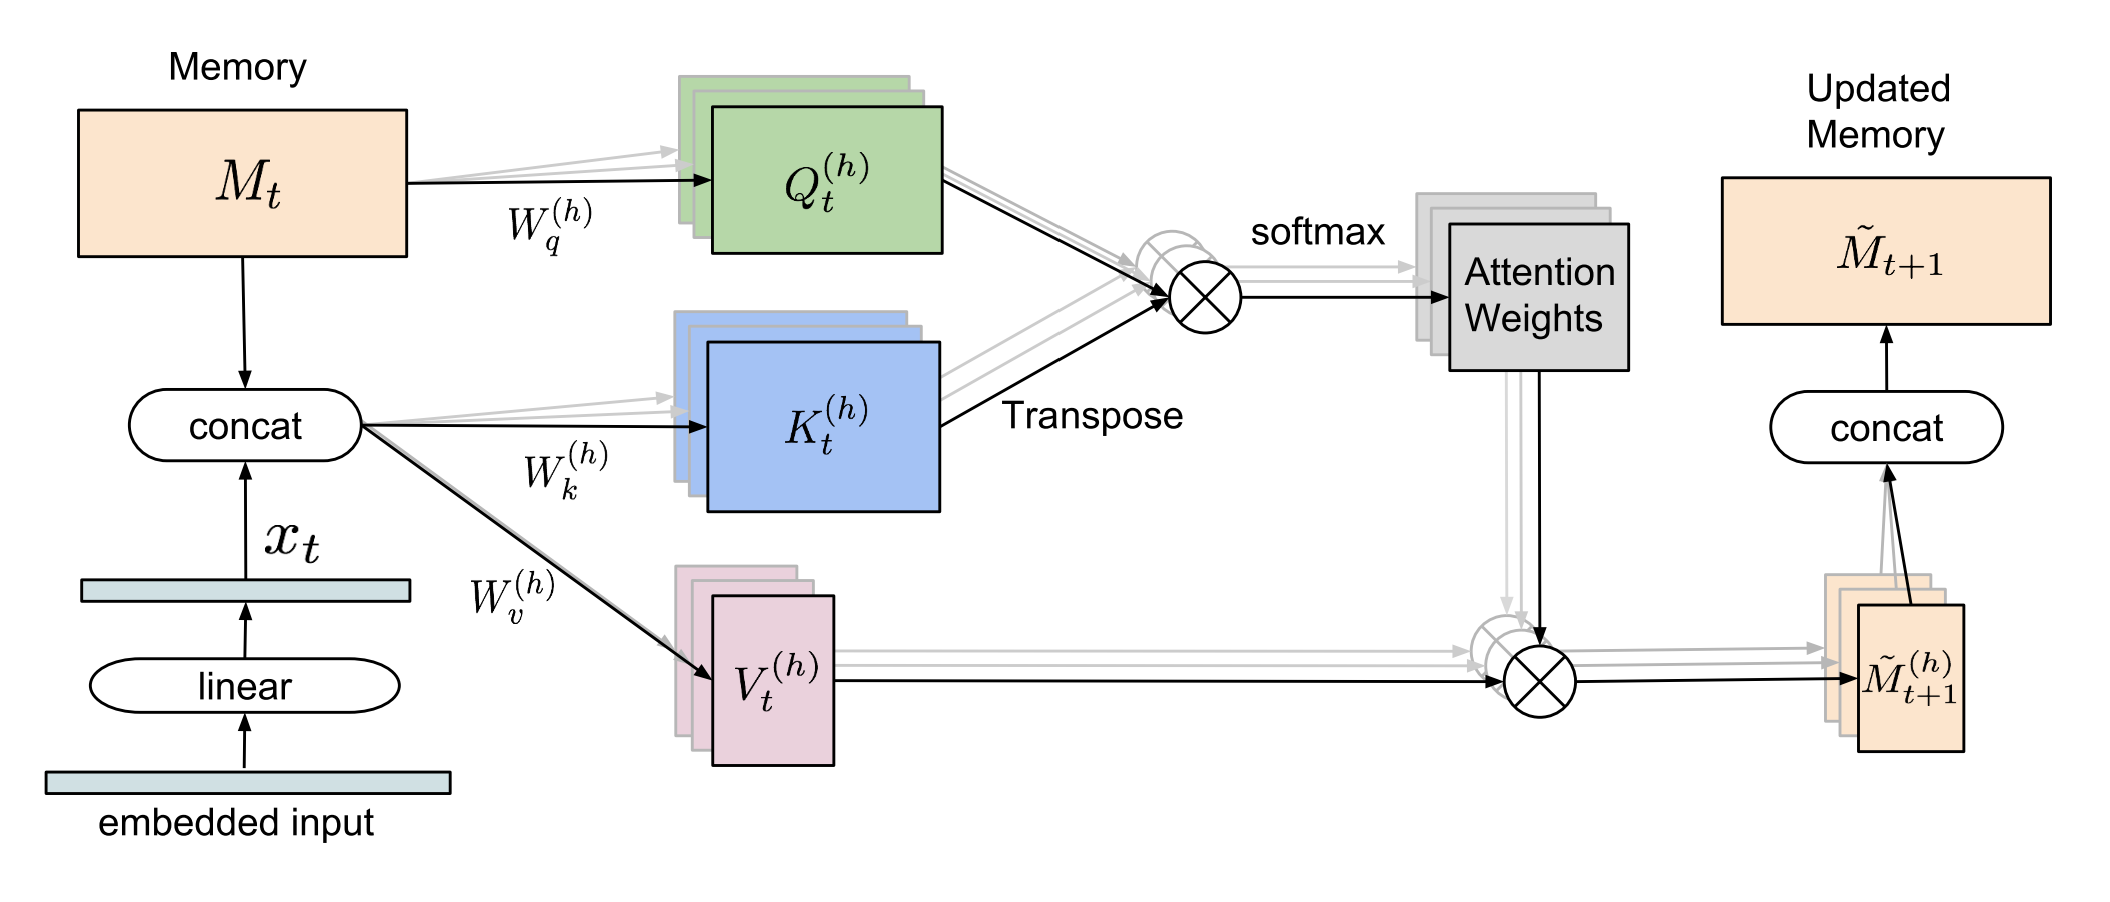
\includegraphics[width=0.8\linewidth]{Images/RelationalMemorySelfAttention.png}
		\caption{Relational Memory with Self-Attention Model}
		\label{img:RelationalMemory}
	\end{figure}
	
	\textit{Qua secondo me bisogna andare più nel dettaglio di cosa si fa effetivamente dentro una Relational Memory con anche formule etc perchè servono dopo per spiegare l'output del modello.}
	
	\item \textit{Gumbel-Softmax Relaxation}: This is the method that RelGAN uses to sample from the output distribution of the generator. As stated before in this discrete data environment it is important to have a one-hot like vector as output and many techniques were invented to deal with this problem. This is a technique used to sample from a distribution. The problem is that sampling from a multinomial distribution can be done using \myeqref{eq:ArgmaxSampling}.
	
	\begin{equation} \label{eq:ArgmaxSampling}
	y_{t} = one\_hot(arg max(o_{t})) 
	\end{equation}
	
	However, it is not possible to pass the gradient through the operation of argmax because it is not drivable. For this reason some techniques, such as Gumbel-softmax relaxation, have been invented.
	\begin{equation}
	\begin{split}
	\label{eq:gumbel}
	y_{t} = \sigma(\beta(o_{t} + g_{t})) \\
	g_{t} = -log(-log \; U_{t}) \\
	U_{t} \sim Uniform(0,1)
	\end{split}
	\end{equation}
	where $\sigma(\cdot)$ is a softmax function which is done element-wisely on its argument. \\
	It should also be consider the parameter $\beta$ that is called \textit{temperature} and it can control sample diversity and quality. Larger $\beta$ encourages more exploration to improve the diversity of the output instead smaller values of $\beta$ push to more exploitation, increasing the quality, therefore the Bleu score, conceding something on diversity. 
	\item \textit{Multiple Representation in Discriminator}: A common used discriminator in such cases is a CNN-based classifier for its ability, thanks to filters of different sizes, of collecting information from different relations between elements in the input. In this case the input is a series of one-hot vector $[r_{1} : ... : r_{T}]$ and, as proposed in previous chapter, it is important to have an embedding matrix to capture different concepts around the input sequence. It often happens that the embedding matrix is learnt through gradient propagation by the system in order to have the best possible embedded representation. In this work they propose not have one such structure but many of them in parallel, as show in [Fig \ref{img:MultipleDiscriminator}], in order to allow the network to learn different representation of the words in input. Thanks to the ablation study done at the end of the paper it is clear how this procedure is effective to push the generation forward keeping important information on the context and on the syntax situation of the sentence ($e.g.$ if a comma or a preposition is needed)
		
	\begin{figure}[h!]
		\centering
		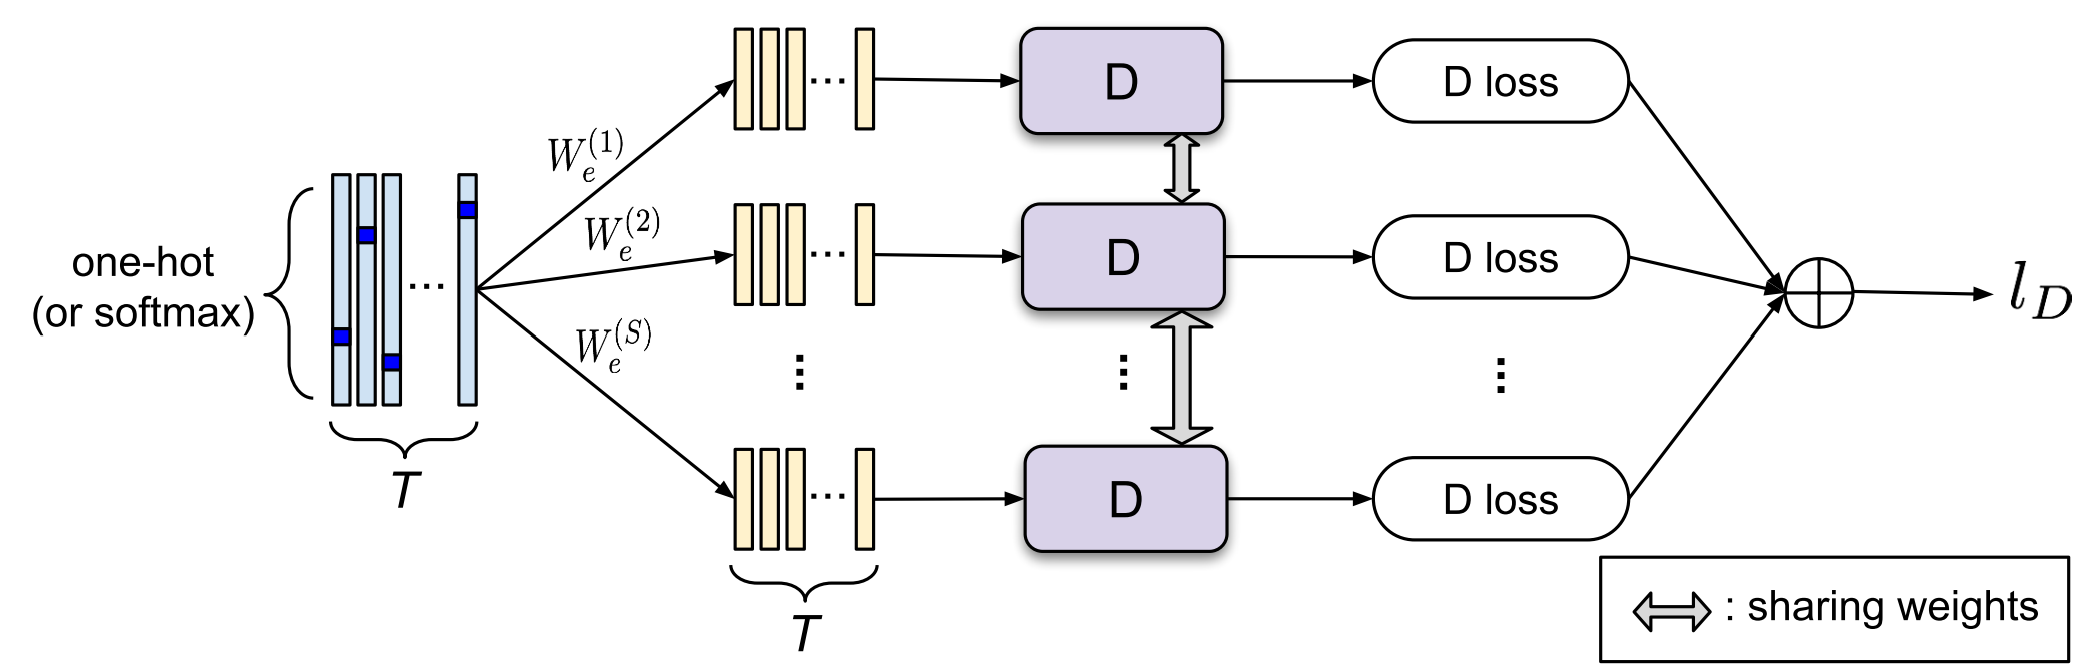
\includegraphics[width=0.8\linewidth]{Images/MultipleDiscriminator.png}
		\caption{Multiple Discriminator}
		\label{img:MultipleDiscriminator}
	\end{figure}
\end{enumerate}

\textbf{
Lot of this work can be based on a Survey done 1-2 years ago \cite{Lu} \\
There there are many other works that speaks about GAN and what I want to point out is that all these works are really new. New in the sense of the last months. \\
This is what I would like to show that everything is based on something really new. \cite{Chen} \cite{DeMasson} \cite{Dieng} \cite{Fedus2018} \cite{RelGAN} \cite{Guo} \cite{Lin2018} \cite{Wang2018} \cite{Yu2016} \cite{Zhang2017} \\
This is not a GAN based model but it is done using Variational Autoencoders \cite{Wang}
}
\subsection{Transformer Based}
Here there could be a big section related to all the works based on language models trained on big corpus like Bert and recent works on GPT by OpenAI

\clearpage

\section{Topic-Guided GANs}
\label{sect:TopicGuidedGANs}
\textit{Here there is the big part on the work that we have done during the thesis. \\
I think this should go through all the steps, the difficulties and the change we did in order to get to the result we'll have at the end. \\
It is important to give a meaning to the whole thesis
\\ \\}
Many of the works presented above (\nameref{sect:TopicRNN}, \nameref{sect:SeqGAN}, \nameref{sect:RelGAN}) are for sure interesting development for what concern pure text generation. However, if you want to take these models to a real world where there is a clear need to integrate the potential of these solutions with humans, it is mandatory to improve these architectures in order to consider a human input and then be able to manipulate the automatic generation of text according to the will of the user. With this in mind, the work aims to move away from the pure text generation towards a model of \textit{conditioned text generation}. This is the idea on which the proposed new architecture is based.

\subsection{Methods}
The most promising paper, at the moment of the beginning of the work, was the \nameref{sect:RelGAN} architecture published at one of the most famous and prestigious conference of Language Representation. For this reason the model is based on that solution. However it was a challenge to understand how to force the generation to create topic specific utterances. \\
The output of the generator at each step is a vector that represent a distribution over the number of words: assuming that the vocabulary size is $V$, the output logits of the generator is $o_{t} \in \R ^{V}$. This output logits come from the relational memory output that was passed through a Linear Layer:
\begin{equation}
o_{t} = f_{\theta_{1}}(M_{t})
\end{equation}


The topic vector model, namely \nameref{sect:LDA}

\subsection{Results}
Here there are the results in which it is compared also with other approaches
\clearpage

\bibliographystyle{IEEEtran}
\bibliography{IEEEabrv,Sections/biblio}
\end{document}
